\documentclass[11pt]{article}
\usepackage{graphicx}
\usepackage{titling}
\usepackage{geometry}
\usepackage{subcaption}
\usepackage{float}

\title{Lab 5 Report}
\author{Chad Lape and Colton Murray}
\date{February 16, 2020}

\graphicspath{{./images/}}

\setlength{\droptitle}{-4em}

\begin{document}
	\maketitle
	\section{Objectives}
	The objective of this lab was to explore the concept of exceptions and templates. These are important aspects of object oriented programming. With templates they help to ensure that code is versatile and can be used later on without being rewritten. Exceptions allow for the code to control how the code runs and which edge cases are not able to be crossed. This is important to the entire field of CS as it helps to prevent bugs and vulnerabilities. 
	\section {Tasks}
	\subsection{Task 1}
	The shelf utilized a first in, last out approach which works well with arrays. We utilized a variable which would count how many items were in the shelf. To add we would first add an object and then move the counter. To remove we would move the counter back and return the object it was on.
	\newpage
	\subsection{Task 2}
	\begin{figure}[H]
		\begin{subfigure}{.5\linewidth}
			\centering
			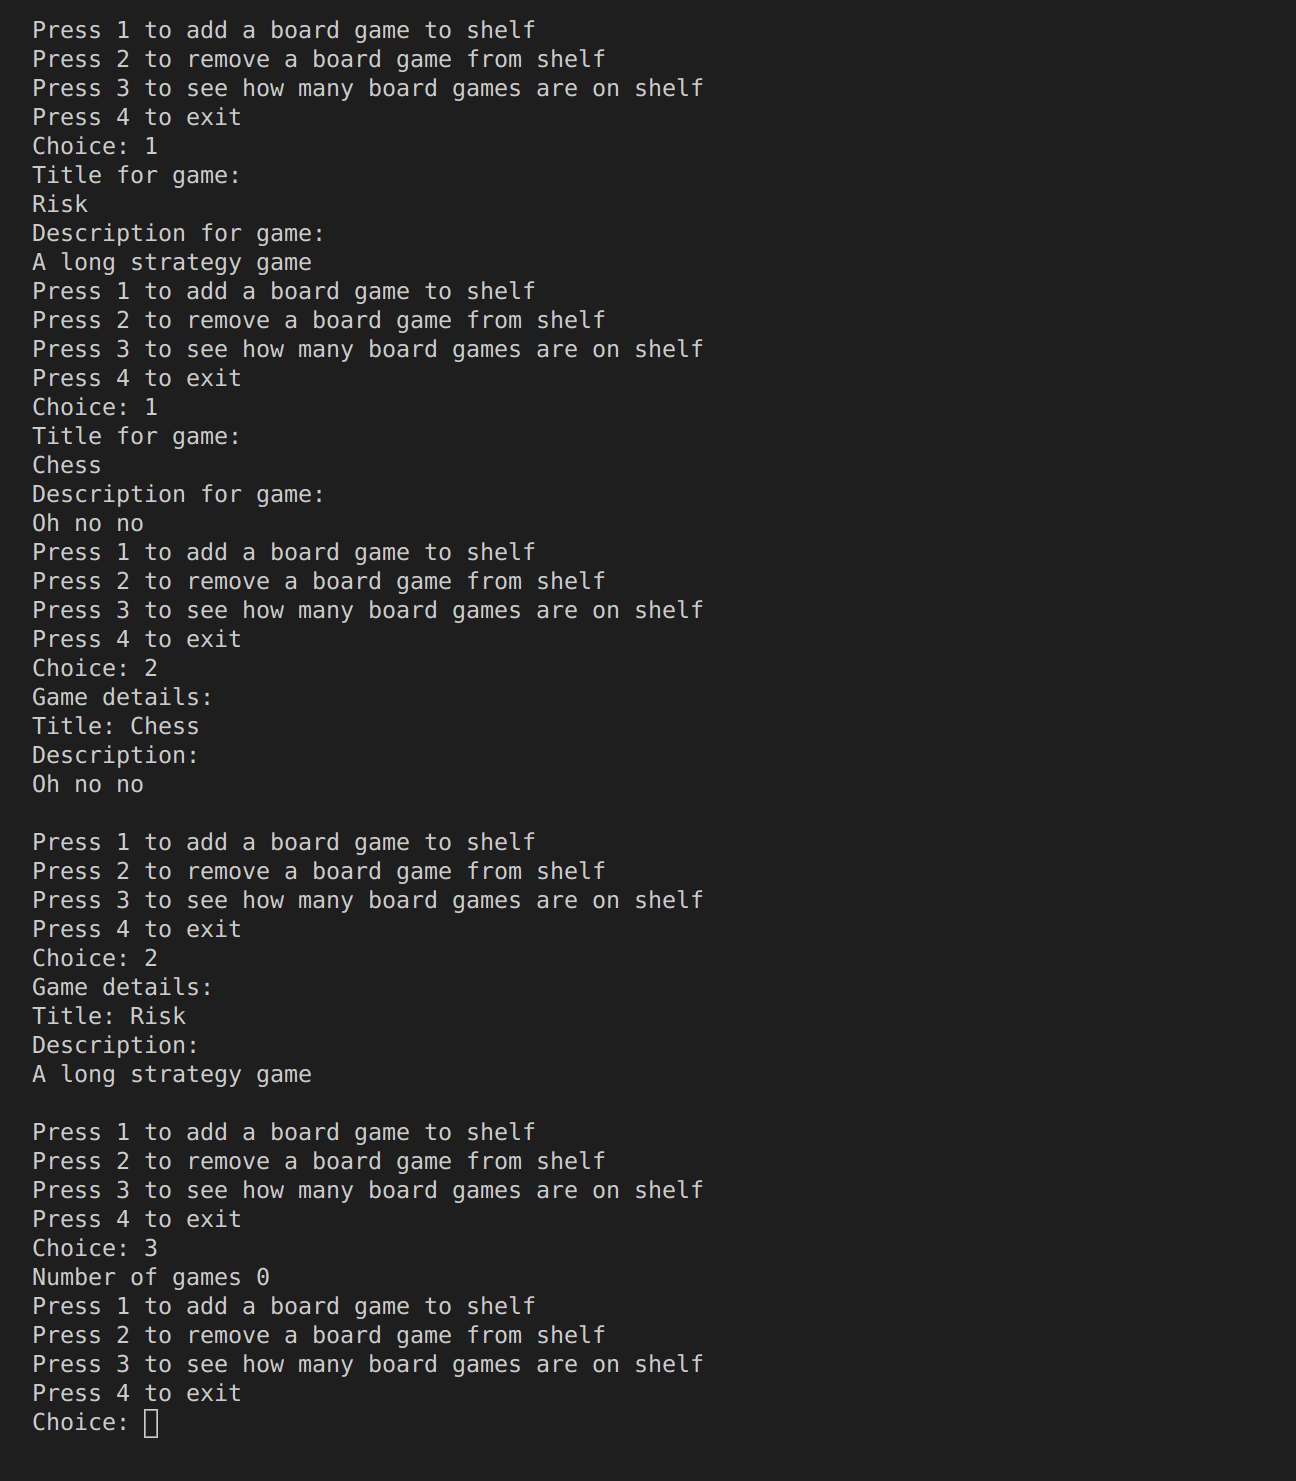
\includegraphics[scale=0.5]{Task2p1}
		\end{subfigure}
		\begin{subfigure}{.5\linewidth}
			\centering
			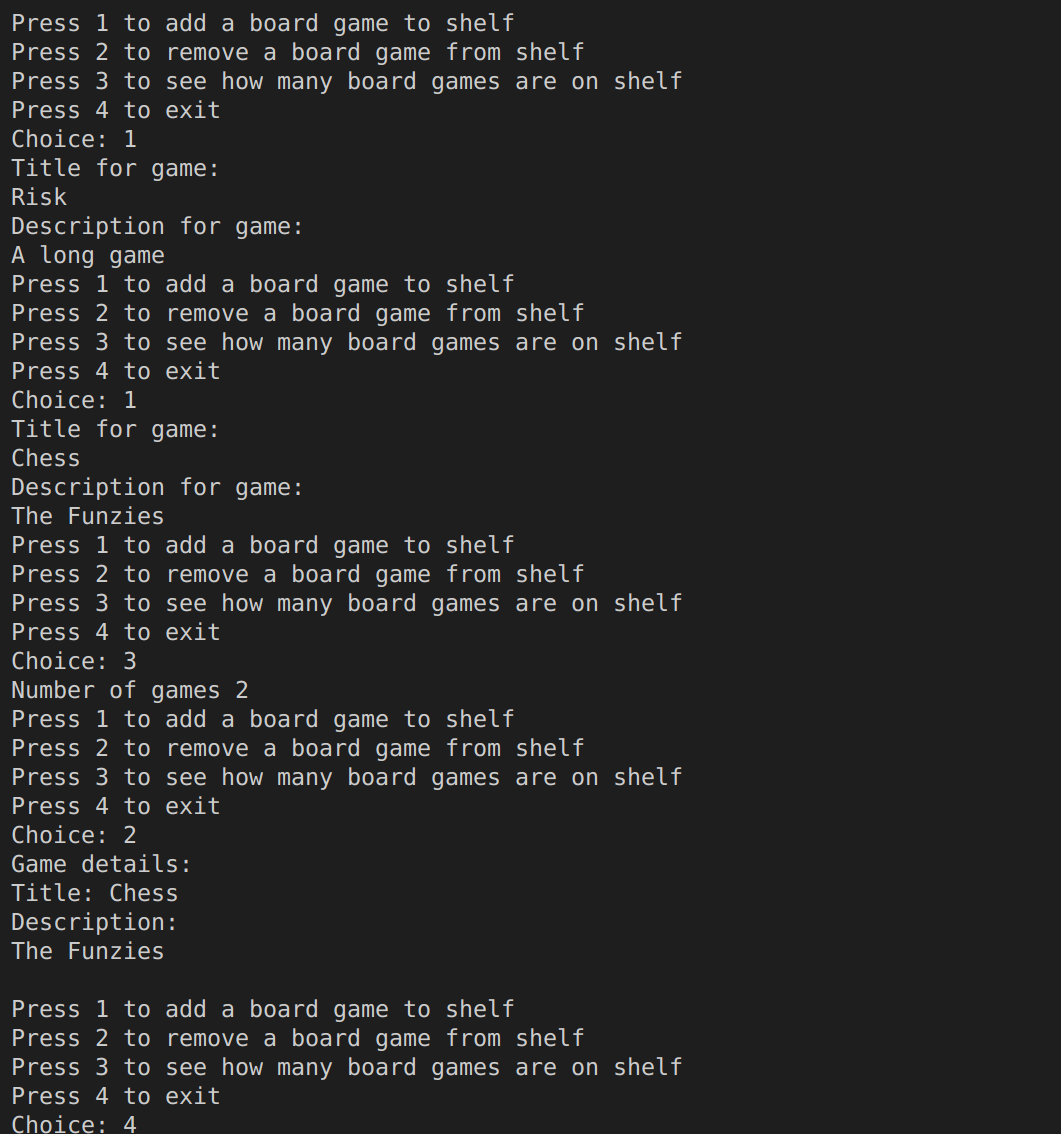
\includegraphics[scale=0.6]{Task2p2}
		\end{subfigure}
	\caption{Using the Shelf Class}
	\end{figure}

	\subsection{Task 3}
	The advantage of trapping an error in a class is that if there is a default way of handling the error then this would always occur. This also means that code would not need to rely on its implementer to function without passing an exception. This can help the program to still function after the user performs an action which was unexpected.
	\begin{figure} [H]
		\begin{subfigure}{0.6\linewidth}
			\centering
			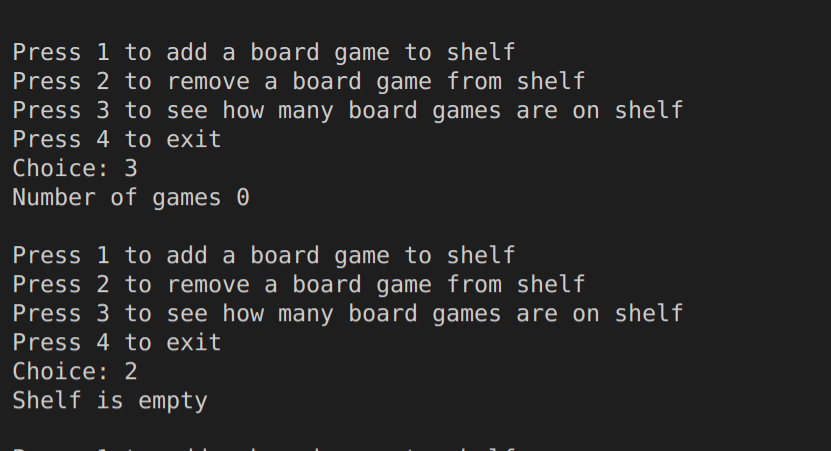
\includegraphics{Task3empty}
			\subcaption{Empty Exception}
		\end{subfigure}
		\begin{subfigure}{0.4\linewidth}
			\centering
			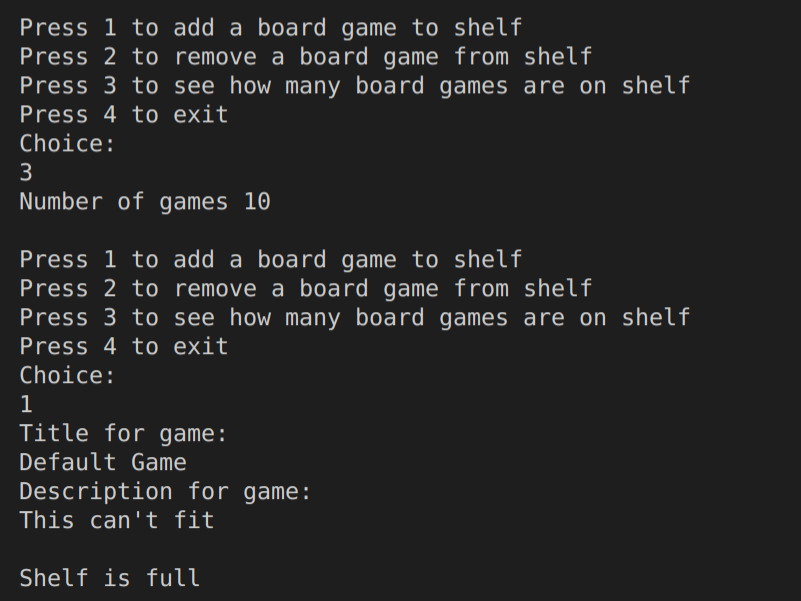
\includegraphics[scale=0.8]{Task3Full}
			\subcaption{Full Exception}
		\end{subfigure}
	\caption{Task 3 Screenshots}
	\end{figure}
	
	\subsection{Task 4}
	Using a template will save time code as well as ensure that this code remains versitile in the future. It also saves memory space as potentially less code has to be loaded as only what is going to be used is loaded instead of every possible combination. This also allows code to work with user made objects as well and saves the programmer who uses the code time of creating an implementation which works with their code if it works in the general template.
	
	\begin{figure} [H]
		\centering
		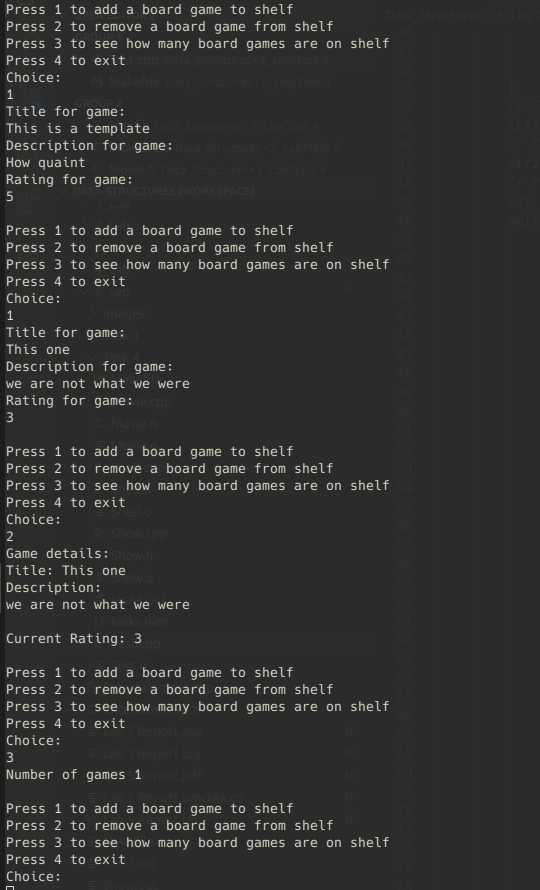
\includegraphics[scale=0.7]{Task4}
		\caption{Task 4 Screenshot}
	\end{figure}

	\section{Conclusion}
	\subsection{Contributions}
	\begin{itemize}
		\item [Chad]
		\begin{itemize}
			\item Created Shelf Declaration
			\item Created Testing Function
			\item Implemented Template Class
			\item Created Lab Report
		\end{itemize}
		\item [Colton]
		\begin{itemize}
			\item Created Shelf Implementation
			\item Created Initial Template Class
			\item Assisted Testing Function
		\end{itemize}
	\end{itemize}
	\subsection{Compiling}
	All the code is precompiled into a windows executable. However in the event that fails to run it can be compiled with a mingw g++ compiler or by throwing it into Visual Community. If those do not work please contact Chad with any issues.

\end{document}